\chapter{Einleitung}
%Begonnen werden soll mit einer Einleitung zum Thema: z.B. Hintergrund und Ziel
%(was, warum).
In vielen Computerspielen ist eine Funktion von N�ten um Einheiten und Charaktere ans Ziel zu f�hren. Egal in welchen Genre, wenn sich der Computer in einer simulierten Umgebung effizient zurecht finden soll, wird ein Wegfindealgorithmus ben�tigt. Um Umwege und unnat�rlich wirkendes Verhalten zu vermeiden, bietet sich ein heuristischer, Graphen basierter Algorithmus an.
Dieser hat sich als effizienteste L�sung f�r Wegfindeprobleme erwiesen.\\
Nicht nur in Civilization, wo die Funktionsweise dem Spieler als ein Zentrales Spielelement bewusst wird, finden solche Algorithmen Verwendung. Auch Genres scheinbar abseits taktischer Tiefe, wie Beispielsweise MMORPGS oder Shootern w�ren ohne dieselben nicht realisierbar.\\

%In vielen Jahren der Spieleentwicklung hat sich A*(A-Stern) als der Effizienteste seiner Art herauskristallisiert.
Wegen seiner einfachen Implementierung und seines hohen Effizienzgrades hat sich A*(A-Stern) als Geeignetster seiner Art bew�hrt. Daher wird heute kaum noch auf andere L�sungen zur�ckgegriffen um entsprechende Probleme zu bew�ltigen. In so fern wird sich diese Arbeit mit den Eigenschaften und der Umsetzung in Programmen von A* befassen.

\chapter {Dijkstra}
Dijkstra bildet die Grundlage zu A*. Er wurde vom gleichnamigen Professor im Jahr 1959 in einem Lehrbuch erl�utert.\footnote{\cite{EWD:NumerMath59}} Es ist der �blichste Algorithmus, der sowohl f�r Netwerkrouting eingesetzt wird, als auch f�r Kartennavigationsger�te.\footnote{\cite{tanenbaum:CN}} //

D
\begin{figure} %[hbtp]
	\centering
		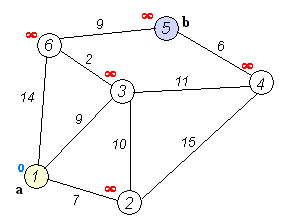
\includegraphics{images/Dijkstra-Beispiel/0.png}
	\caption{Bezeichnung der Abbildung}
	\label{Schritt1}
\end{figure}

-A*
-D*?
